\chapter{Preliminaries}

This chapter makes precise what most of the jargon that appears in our parameterized analysis of complexity means.
The chapter is split into two parts, the second of which, Section~\ref{sec:framework}, should not be skipped in a first reading.
In that section, we introduce a novel framework for parameterized complexity theory, building on the frameworks discussed in Section~\ref{sec:parameterized_complexity_theory}.
All of the theory in Chapter~\ref{ch:parameterizations} will be developed in this new framework.
We remark that many of our results are independent of the framework they are expressed in.
However, using one of the traditional frameworks of Section~\ref{sec:parameterized_complexity_theory} may make the theorems less general, or at the least less elegant.
A brief summary of the notation that is specific to our framework can be found in the back of this thesis.

The first part of the current chapter, Section~\ref{sec:established_theory}, does not contain anything not available in textbooks.
We have divided it into subsections corresponding to particular research areas.
While the section does include some background on our usage of certain terms, it, or segments of it, may be skipped at will or used only as a reference.
The numbers of the pages on which definitions are listed can be found in the index at the back of this thesis.


\bigsection{Established Theory}
\label{sec:established_theory}%

We aim to bring together multiple notions of complexity.
It is unavoidable that, in doing so, we use terminology from multiple areas of research.
Broadly, each section of Chapter~\ref{ch:parameterizations} deals with a form of complexity as it is encountered in a specific area of research.
Definitions that are specific to a certain area of research are stated in the appropriate sections.
More basic definitions that span multiple areas of research are included here.
While we accompany all definitions with some context, we cannot give a complete introduction to each of the research areas that we draw definitions from.


\subsection{Binary Representations}
\label{sec:preliminaries:binary}%

In this thesis, as in much of the computer science literature, all sets are countable.
That means that for every set~$A$, there exists a surjective function mapping the natural numbers, $\bbN \deq \{1, 2, 3, \ldots\}$ onto~$A$.
The elements of a countable set can be represented by finite \emph{strings} of characters from a finite \emph{alphabet}.
We shall work solely with the binary alphabet~$\binary \deq \{\bits{0}, \bits{1}\}$, but all results can be generalized to more elaborate alphabets.
The finite, nonempty binary strings, $\binary^+$, can be enumerated in order of increasing length as $\bits{0}, \bits{1}, \bits{00}, \bits{01}, \bits{10}, \ldots$.
Thus, there is a bijective correspondence between $\bbN$ and~$\binary^+$.
Taking a cue from common practice in programming languages, we treat the two directions of this bijective correspondence as data type conversions.
A string can serve \enquote{as an integer}, that is \enquote{as a natural number}, and a natural number can serve \enquote{as a string}.
These data type conversions are depicted in Table~\ref{tab:cast}.
In this thesis, we have tried to make all conversions explicit.

\begin{table}[htbp]
  \centering
  \vspace*{3ex}
  \begin{tabular}{c@{\hspace{3cm}}c}
    \clap{\tikz[remember picture] \node (N) {$\bbN$};} & \clap{\tikz[remember picture] \node (binary) {$\binary^{\mathrlap{+}}$};} \\[4ex]
    $1$ & \bits{\phantom{00}0} \\
    $2$ & \bits{\phantom{00}1} \\
    $3$ & \bits{\phantom{0}00} \\
    $4$ & \bits{\phantom{0}01} \\
    $5$ & \bits{\phantom{0}10} \\
    $6$ & \bits{\phantom{0}11} \\
    $7$ & \bits{000} \\
    $8$ & \bits{001} \\
    $\vdots$ & $\vdots$
  \end{tabular}
  \begin{tikzpicture}[overlay,remember picture]
    \path[->,bend left,looseness=0.8,auto]
      (N)      edge node {$\asStr$} (binary)
      (binary) edge node {$\asNat$} (N);
  \end{tikzpicture}
  \caption{
    A bijective correspondence between the natural numbers and the finite, nonempty binary strings.
    The two directions of this correspondence are denoted by $\asStr$ and~$\asNat$.
    Note that the number~$0$ and the empty string are never used in this thesis.
  }
  \label{tab:cast}
\end{table}

We have chosen to forego any consideration of the empty string and, in this thesis, we do not consider $0$ to be a natural number.
Of course, these choices are related to each other and make that the set of possible lengths of our strings equal the set of natural numbers.
Our choices ensure that any statement about a natural number that is true \enquote{up to an additive constant} is also true \enquote{up to a multiplicative constant}.
Let us give an example.
If, given two natural numbers $x$ and~$y$, there is a constant $c$ such that we have $x \le y + c$, then there is also a constant $c'$ such that we have $x \le c \cdot y$.
The fact that this need not be the case if $x$ was equal to $0$ makes that $0$ is often a special case that needs special treatment.
By leaving out $0$ from the start, we are not bothered by these pathological cases.

The elements of~$\binary$ are known as \emph{bits}.
The number of bits in a binary string~$x$ is called the \emph{length} of~$x$ and denoted by~$\length{x}$.
We denote the set of all strings of some length~$n$ by~$\binary^n$.
Observe that for any two natural numbers $m$ and~$n$, we have
\begin{equation*}
  m \le n \implies \length{\asStr(m)} \le \length{\asStr(n)}.
\end{equation*}
Furthermore, we implicitly take all our logarithms to base~$2$.
This ensures that $\log n$ is within one bit of $\length{\asStr(n)}$.
By not being pedantic about this difference of at most one bit, we can say that $n$~elements can be distinguished from one another using $\log n$~bits.

Two strings $x$ and~$y$ can be concatenated to form a new string.
This concatenation of $x$ and~$y$ is written simply as $xy$.
Note that we have $\length{xy} = \length{x} + \length{y}$.
The $n$-fold concatenation of $x$ with itself is written as $x^n$.
In particular, we have
\begin{equation*}
  \bits{0}^n = \underbrace{\bits{000}\cdots\bits{0}}_{\text{$n$ copies of \bits{0}}}.
\end{equation*}

Given the concatenation of two strings, we cannot recover the two original strings.
Indeed, an equation like $\bits{010111001} = xy$ has no unique solution.
We do not know what initial segment, or \emph{prefix}, of~\bits{010111001} corresponds to~$x$.
If we want to be able to recover the components in a composite string, we cannot simply concatenate them.
\begin{definition}
  Let $\Omega$ be any set.
  An injective function $f\colon \Omega \to \binary^+$ is a \emph{prefix-free encoding} of~$\Omega$ if there are no two distinct elements $\omega_1$ and~$\omega_2$ of $\Omega$ such that $f(\omega_1)$ is a prefix of $f(\omega_2)$.
\end{definition}

With a suitable application of a prefix-free encoding of binary strings, it is possible to uniquely decompose a composite string~\parencite{cover2006elements}.
Perhaps the simplest prefix-free encoding of binary strings is the \emph{unary encoding}, where the position of the first~\bits{1} determines the encoded string.
The unary encoding of a binary string~$x$ is
\begin{equation*}
  \unary(x) \deq \bits{0}^{\asNat(x) - 1} \bits{1}.
\end{equation*}
Note that the unary encodings of any two distinct strings are different and that the unary encoding of a string always ends at the first occurrence of~`\bits{1}'.
Therefore, unary encoding is indeed a prefix-free encoding of~$\binary^+$.
Contrary to the situation we were in with direct concatenation, the equation $\bits{010111001} = \unary(x)y$ \emph{does} have a unique solution.
Namely, it has the solution $x = \asStr(2) = \bits{1}$ and $y = \bits{0111001}$.

Unary encoding comes with a substantial blow-up in the length of a string.
For any string~$x$, we have $\length{\unary(x)} = \asNat(x)$, which is exponential in~$\length{x}$.
More frugal prefix-free encodings were developed by \textcite{elias1975universal}.
The two most famous of these are known as \emph{Elias~gamma coding} and \defkey{Elias~delta coding} \parencite[see also][]{sayood2017introduction}.
In Elias~gamma coding, a string is prefixed by a unary encoding of its length,
\begin{equation*}
  \mathrlap{
    \Elias_\gamma(x) \deq \unary(\asStr(\length{x})) x = \bits{0}^{\length{x} - 1} \bits{1} x.
  }\hphantom{
    \Elias_\delta(x) \deq \Elias_\gamma(\asStr(\length{x})) x = \bits{0}^{\length{\asStr(\length{x})} - 1} \bits{1} \asStr(\length{x}) x.
  }
\end{equation*}
Thus, the position of the first occurrence of~`\bits{1}' tells us how many of the following bits make up the encoded string~$x$.
So, the equation $\bits{010111001} = \Elias_\gamma(x)y$ has the unique solution $x = \bits{01}$ and $y = \bits{11001}$.

With Elias~gamma coding, we have $\length{\Elias_\gamma(x)} = 2 \cdot \length{x}$.
The same trick underlying Elias~gamma coding can be used to bring the length of the encoding of~$x$ even closer to~$\length{x}$.
In Elias~delta coding, we replace the unary encoding of the length of~$x$ by an Elias~gamma encoding of that length,
\begin{equation*}
  \Elias_\delta(x) \deq \Elias_\gamma(\asStr(\length{x})) x = \bits{0}^{\length{\asStr(\length{x})} - 1} \bits{1} \asStr(\length{x}) x.
\end{equation*}
For a string~$x$ of length~$n$, this gives us $\length{\Elias_\delta(x)} = 2 \cdot \length{\asStr(n)} + n$, which is approximately $n + 2 \cdot \log n$.

For our purposes, Elias~delta coding is sufficiently economical.
We shall use it whenever we need to pair strings.
\begin{definition}
\label{def:pairing_function}%
  A \emph{pairing function} that combines two finite, nonempty binary strings $x$ and~$y$ into a single string is given by
  \begin{equation*}
    \pair{x}{y} \deq \Elias_\delta(y)x.
  \end{equation*}
\end{definition}

Note that this pairing function reverses the order in which the components are presented.
There is no fundamental reason for this technical detail other than that it will be convenient in Example~\ref{ex:traditional_pc} and in Section~\ref{sec:statistics} in general.
Returning to our example string one final time, we observe $\bits{010111001} = \Elias_\delta(\bits{1100})\bits{1}$ and hence $\bits{010111001} = \pair{\bits{1}}{\bits{1100}}$.

Our pairing function does not use any prefix-free encoding for its first component.
This has the effect that our pairing function is not a prefix-free encoding of~$\binary^+ \times \binary^+$.
At the same time, it results in $\length{\pair{x}{y}}$ being approximately equal to $\length{x} + \length{y} + 2 \cdot \log \length{y}$.

Prefix-free encodings have an interesting relation to probability theory.
The length of the prefix-free encoding of a string can be linked to the probability of that string in some probability mass function~\parencite{cover2006elements,li2008introduction}.
\begin{theorem}[Kraft~inequality\indexkey{Kraft~inequality}]
  If $f$ is a prefix-free encoding of a set~$\Omega$, then we have
  \begin{equation*}
    \sum_{\omega \in \Omega} 2^{-\length{f(\omega)}} \le 1.
  \end{equation*}
  Conversely, if there is a function~$\ell\colon \Omega \to \bbN$ that satisfies $\sum_{\omega \in \Omega} 2^{-\ell(\omega)} \le 1$, then there is a prefix-free encoding~$f$ of~$\Omega$ such that, for all $\omega$, we have $\length{f(\omega)} = \ell(\omega)$.
\end{theorem}
Thus, the quantity~$2^{-\length{f(\omega)}}$ acts like a probability of~$\omega$.
For technical reasons, the probability mass function is allowed to sum to less than~$1$ in the Kraft~inequality.
This can be fixed by either normalization, or by introducing a \enquote{slack object} that takes the remaining probability.


\subsection{Algorithmic Complexity and Computability Theory}

We take a pragmatic approach to computability theory and do not consider physical computers to be approximations of Turing machines.
Instead, we consider Turing machines to be asymptotically correct mathematical models of physical computers.
Our model of effective computation hence takes the form of \enquote{reasonable} \emph{pseudocode}.
That is, a programming language that is more or less obviously Turing complete, yet not stronger than that.
A more traditional, but up-to-date textbook on Turing computability is the textbook by~\textcite{soare2016turing}.

With pseudocode, we can specify an \emph{algorithm}, which represent the workings of a particular Turing machine \parencite[see also][]{rogers1967theory}.
We shall not concern ourselves with the details of our pseudocode-language.
Instead, we accept that it is possible to specify such a language in sufficient detail, and assume that we have an effective prefix-free encoding of algorithms.
We shall refer to an encoded algorithm as a \emph{procedure}.
Note that a procedure~$\phi$ has a length~$\length{\phi}$, which is measured in bits.

As algorithms may take input and produce output, they implement partial functions.
The functions they implement may be partial functions, because, for a given input, an algorithm may keep running forever and never settle on any output.
When an algorithm terminates on all possible inputs and the associated function~$f$ is hence a total function, we say that $f$ is \emph{computable}.

Algorithmic complexity theory looks at procedures that generate a given string.
The most widely used measure of algorithmic complexity is \emph{Kolmogorov complexity}~\parencite{cover2006elements,li2008introduction,downey2010algorithmic}.
\begin{definition}
  The \defkey{Kolmogorov complexity} of a string $x$ is
  \begin{equation*}
    \KC(x) \deq \min\{\length{\phi} \st \text{procedure $\phi$ produces $x$ when not provided with any input}\}.
  \end{equation*}
\end{definition}

The precise value of the Kolmogorov complexity of a string depends on the prefix-free encoding of algorithms that is used.
However, Kolmogorov complexity enjoys an invariance theorem, stating that this dependency is limited to an additive constant \parencite[see, for instance][]{li2008introduction}.
In order not to blur the main ideas in this thesis, we shall not write \enquote{up to an additive constant} after every (in)equality involving Kolmogorov complexity.
This is left implicit.

Complexity theory, on the other hand, looks at procedures that output a single bit, either~\bits{1} or~\bits{0}.
If a procedure outputs a single bit and does so on all possible input strings, it is said to be a \emph{decision procedure}.
A decision procedure~$\phi$ \emph{decides} on membership in the set
\begin{equation*}
  A = \{x \st \phi(x) = \bits{1}\}.
\end{equation*}
In turn, the set~$A$ is said to be \emph{decidable}.
If the procedure~$\phi$ fails to halt on some inputs, the set $A = \{x \st \phi(x) = \bits{1}\}$ is said to be \emph{semidecidable}.
The semidecidable sets are more commonly known as the \enquote{recursively enumerable} sets.
However, we prefer to use the word \enquote{recursive} only for the algorithmic design pattern by that name.
We do note that the semidecidable sets can equivalently be defined as those sets of which the members can be enumerated effectively.

The class of semidecidable sets contains sets that are not in the class of decidable sets.
Moreover, not all sets are semidecidable.
In fact, a set can be highly dissimilar to all semidecidable sets at once.
\begin{definition}
\label{def:bi-immune}%
  A set $A$ is \emph{immune} for a class of sets~\cl{\itshape C} if no infinitely large member of~\cl{\itshape C} is a subset of~$A$.

  A set $A$ is \defkey{bi-immune} for a class of sets~\cl{\itshape C} if both $A$ and its complement are immune for~\cl{\itshape C}.

  If no specific mention of a class of sets~\cl{\itshape C} is made, the class implicated is that of the semidecidable sets \parencite{rogers1967theory,odifreddi1992classical}.
\end{definition}
Immune sets where introduced to computability theory by~\textcite{post1944recursively}.
The application to arbitrary classes of sets goes back to~\textcite{flajolet1974sets}.

If the class \cl{\itshape C} in Definition~\ref{def:bi-immune} has infinitely many infinitely large members, an immune set~$A$ satisfies infinitely many requirements.
Namely, for every infinitely large set $C$ in \cl{\itshape C}, the set~$A$ is so that $C \setminus A$ is nonempty.
In many cases, constructing a set that meets infinitely many of such requirements is not straightforward.
It may be complicated by the fact that satisfying one requirement may violate satisfying a requirement that was taken care of earlier.
By imposing a priority ordering on the requirements and always choosing to satisfy the requirement with the highest priority, immune sets can be constructed.
This construction method is known as the \emph{finite injury priority method} \parencite[for details, see][Section~2.11]{downey2010algorithmic}.

By a slight stretch of notation, we may use a set as a function.
The function associated with a set~$A$ is defined as
\begin{equation*}
  A(x) \deq \begin{cases}
    \bits{1} & \text{if $x \in A$}, \\
    \bits{0} & \text{otherwise}.
  \end{cases}
\end{equation*}
Thus, a set is decidable when the function associated to it is computable.
Moreover, a procedure that implements the function associated with a set~$A$ is a decision procedure for~$A$.
In case a set~$A$ is not decidable, we can investigate what would happen if it were decidable, by supposing the function associated with~$A$ is computable.
In particular, we consider the sets that \enquote{become decidable} when this function is computable~\parencite{rogers1967theory,odifreddi1992classical,soare2016turing}.
\begin{definition}
\label{def:reduction:turing}%
  A set~$B$ is \emph{Turing reducible} to a set~$A$ if there is an algorithm that
  \begin{itemize}
  \item is allowed to evaluate the function associated with~$A$, and
  \item decides on membership in~$B$.
  \end{itemize}

  Such an algorithm is known as a \defkeyat{reduction!Turing}{Turing reduction}.
  The set~$A$ is known as an \emph{oracle} and the evaluations of the function associated with~$A$ are known as \emph{queries}.
\end{definition}

The behavior of a Turing reduction may be heavily reliant on the oracle.
Specifically, at any point in its execution, the outcomes of the queries it has made so far may influence the query it makes next.
If a Turing reduction is allowed to have such a dependence on the outcomes of queries, it is said to be \emph{adaptive}.
Sometimes, it is desirable to consider reducibility where the queries are independent of the oracle.
\begin{definition}
\label{def:reduction:truth-table}%
  A set~$B$ is \emph{truth-table reducible} to a set~$A$ if there is a Turing reduction~$\phi$ from~$B$ to~$A$ such that
  \begin{itemize}
  \item the queries made by~$\phi$ depend only on its input and not on the oracle, and
  \item $\phi$ terminates on all inputs, regardless of the oracle.
  \end{itemize}

  Such a Turing reduction is known as a \defkeyat{reduction!truth-table}{truth-table reduction}.
\end{definition}

For a given input to a truth-table reduction, we can gather the queries that would be made.
The possible outcomes of these queries can be assembled as rows in a table.
For each row in this table, we can compute the decision on membership that the truth-table reduction would make.
For this reason, reductions of this kind are called truth-table reductions.

The power of a reduction can be restricted further.
A truth-table reduction that always makes precisely one query and outputs the unmodified result of that query is known as a \defkeyat{reduction!many--one}{many--one reduction}.
If there is a many--one reduction from a set~$B$ to a set~$A$, then $B$ is said to be \emph{many--one reducible} to~$A$.


\subsection{Proof Theory}

The Turing machine was developed as a model for computation as it can conceivably be performed by humans~\parencite[Section~9]{turing1937computable}.
In that respect, it is not surprising that computability theory has close ties to proof theory.
After all, proof theory should seek to model what humans could ultimately achieve in terms of reasoning~\parencite[Section~37]{kleene1967mathematical}.
Accomplishments in human computation and human reasoning are intuitively subject to the same intellectual limitations.

The link between computability theory and proof theory has been formalized into what is known as the \emph{Curry--Howard correspondence}, or the \emph{formulas-as-types isomorphism}~\parencite[Section~2.5]{troelstra2000basic}.
This isomorphism draws a parallel between proofs and algorithms.
Just like we have freedom in the choice of a pseudocode-language, there is freedom in the choice of a \enquote{proof language}, or \emph{proof calculus}~\parencite{kleene1967mathematical,troelstra2000basic}.
We did not concern ourselves with the details of our pseudocode-language and neither shall we concern ourselves with the details of proof calculi.
However, at the heart of every proof calculus lies a \defkeyat{formal system}{formal (deductive) system}~\parencite{kleene1967mathematical}, and we shall briefly go over what is involved with such a system.

Typically, expositions of formal systems start with the definition of a \emph{formal language}.
A formal language is a set of finite strings of symbols from some finite alphabet.
The strings in a formal language are called the \emph{well-formed words}, or \emph{well-formed formulas}.
In this thesis, we are only concerned with formal systems of which the formal language is decidable.
\begin{example}
  Suppose we want our formal system to deal with tree structures.
  We then need a way to represent such structures.
  One way to do so is by using the symbols `$($' and `$)$' and `$,$' and `$\ast$'.
  Using these symbols, we can serialize a nested tree structure, with `$\ast$' representing a leaf in the tree.
  The structure of the tree in Figure~\ref{fig:decomposition:tree} would thus be represented by the string \enquote{$((\ast, \ast), \ast, \ast)$}.

  Not all strings consisting of our symbols represent a tree structure.
  For instance, the string \enquote{$()\ast$} has no meaningful interpretation and is therefore not well-formed.
  The set of strings that do represent tree structures is a decidable subset of the set of all strings of our symbols.
\end{example}

The goal of a formal system is to single out a subset of the well-formed formulas that is of some special interest.
For instance, if the formal language is that of propositional logic, we may want to characterize the tautologies.
To this end, a formal system contains a way of deriving well-formed formulas from other well-formed formulas by means of \emph{rules of inference}.
The idea here, is that the subset of interest is closed under these rules of inference.
The rules of inference can be thought of as a set of procedures, where each procedure takes a number of well-formed formulas and produces a new one.
The number of inputs is fixed for each procedure and if the procedure takes no inputs, then it is said to be an \emph{axiom}.
Thus, an axiom is a procedure that produces a well-formed formula.
For the purposes of this thesis, we restrict our attention to formal systems where the rules of inference are represented by a decidable set of procedures.
\begin{example}[continued]
  Suppose that, in our system of tree structures, we want to derive the nonempty binary trees.
  This can be done with one axiom and one other rule of inference.
  The axiom is a procedure that takes no inputs and outputs the minimal binary tree, the tree with a root node and no branches: \enquote{$\ast$}.
  The other rule of inference is a procedure that transforms two tree structures, $x$ and~$y$, into the tree structure~\enquote{$(x, y)$}.
  Using these two rules of inference, all binary trees can be derived, and nothing else.
  For example, it is impossible to generate our earlier example, \enquote{$((\ast, \ast), \ast, \ast)$} using only these two rules, because it does not represent a binary tree.
\end{example}

A \emph{proof}, or \emph{deduction}, in a formal system establishes that some given well-formed formula~$x$ is part of the subset of special interest.
It does so by specifying a sequence of rules of inference that, together, output~$x$.
Thus, the proof constructs~$x$ from the axioms of the formal system.

In this thesis, we are only ever interested in the well-formed formulas of a formal language.
This is most notable in how we approach decision problems.
For example, when we model a graph-theoretic decision problem as a set of graphs, we expect the input to a decision procedure for the set to be a graph.
We pay no attention to what would happen if the input does not represent a graph.
In fact, we shall routinely assume that there is some computable bijection between the well-formed formulas and the binary strings,~$\binary^+$.
A decision procedure for a graph problem can then be provided with a binary string as input, and we can act as if it was given a graph.
To hide this conceptual difference between well-formed formulas and binary strings, we shall refer to the input of a decision procedure as a problem \emph{instance}.
Put differently, in the context of a decision problem modeled as a set, an instance is a syntactically correct specification of a potential member of the set.
Where the details of the encoding of well-formed formulas as binary strings matter, we shall be explicit about the encoding we use.


\subsection{Computational Complexity Theory}

Our choice of using pseudocode-algorithms as a model of computation does not mean that our results are limited to that particular model of computation.
Many other models of computation identify the exact same class of partial functions as computable.
The Church--Turing thesis asserts that this class includes effective computation by an idealized human, in some intuitive, informal, sense~\parencite{vanemdeboas1990machine,goldreich2008computational}.
However, the Church--Turing thesis does not imply that \emph{all} our results extend to all models of computation that are equivalent to the Turing machine.

We have mentioned that the precise value of the Kolmogorov complexity of a string depends on the prefix-free encoding of algorithms that is used.
This dependence is limited to an additive constant by the existence of a \emph{universal} procedure that takes a procedure~$\phi$ and string~$x$ as inputs, and outputs~$\phi(x)$~\parencite{li2008introduction,goldreich2008computational}.
Likewise, the dependence of Kolmogorov complexity on the model of computation is limited to an additive constant, as long as the models can simulate each other.
This idea is made precise by \textcite{rogers1967theory} in the form of \emph{acceptable numberings} of partial computable functions \parencite[see also][]{soare2016turing}:
When a model of computation corresponds to an acceptable numbering of functions in our reference model, its notion of Kolmogorov complexity equals ours.
Equivalently, all models of computation that are equivalent to the Turing machine and have a universal procedure share a notion of Kolmogorov complexity.

There is no canonical representation, or, for that matter, formal definition, of a computational procedure by an idealized human.
Therefore, the Church--Turing thesis does not entail that Kolmogorov complexity coincides with some intuitive human understanding of algorithmic complexity.
Additionally, it does not entail that in different models, the same functions can be computed in the presence of a given bound on some computational resource.
Indeed, an analysis of the resource requirements for computing a given function need not transcend the model of computation that is used.

The main computational resource we look at in this thesis is the number of steps taken by an algorithm, referred to as computation \emph{time}.
To more cleanly express the asymptotic behavior of computation-time usage, computation time is commonly measured as a function of the length of input instances.
That is, the computation time of a procedure~$\phi$ is a function~$t$ such that, for all~$n$, the maximum number of steps taken by~$\phi$ on any input of length~$n$ is $t(n)$.
Typically, it is not so much the exact computation time of a procedure we are interested in, but rather an upper bound on the computation time.
When we say that a procedure~$\phi$ runs in time~$t$, we mean that, for all~$n$, the number of steps taken by~$\phi$ on any input of length~$n$ is at most~$t(n)$.
A noteworthy class of functions in this regard are the \defkeyat{time-constructible function}{time-constructible functions}.
These are the functions~$t$ for which there is a procedure~$\phi$ and a constant~$c$ such that, for all strings~$x$,
\begin{itemize}
\item $\phi$ outputs the string representation of $t(\asNat(x))$ on input $x$, and
\item $\phi$ takes at most $c \cdot t(\length{x})$ steps on input $x$.
\end{itemize}
Most commonly used functions, among which all polynomials of degree at least~$1$, are time-constructible~\parencite{arora2009computational}.

Many models of computation that have been studied can simulate each other with only polynomially-bounded overhead in computation time~\parencite{vanemdeboas1990machine}.
In fact, it has been conjectured that, for some definition of \enquote{reasonable}, all reasonable machines can simulate each other with polynomially-bounded overhead.
This extension to the Church--Turing thesis is, among other names, known as the \emph{sequential computation thesis}.
The name reflects the fact that the thesis is found to exclude some parallel models of computation~\parencite{parberry1986parallel,vanemdeboas1990machine}.
We shall not be concerned with whether or not the sequential computation thesis is true in general, but we shall assume a special case.
As argued by \textcite{turing1937computable}, the idealized human computer may be thought of as a sequential model of computation.
We accept these arguments to the extent that the sequential computation thesis can be applied to the idealized human computer.
In particular, we assume that the idealized human computer and our model of computation can indeed simulate each other with polynomially-bounded overhead.
Like the Church--Turing thesis, this statement is necessarily informal.
Specifically, there is no formal definition of what a single computational step of a human computer would be.

The sequential computation thesis is especially relevant in light of yet another thesis on the computational abilities of the idealized human computer.
Around 1965, Cobham and Edmonds argued that the functions that should be called \emph{efficiently computable} are those that can be computed in polynomial time \parencite[see also][]{goldreich2008computational}.
Thanks to the sequential computation thesis, efficient computability is a somewhat robust notion.
We may assume that what is efficiently computable in our model of computation is also efficiently computable for the idealized human computer and vice versa.

The class of sets that have efficiently computable decision procedures in our model of computation is denoted by~\cl{P}.
For other models of computation, the class of sets that have efficiently computable decision procedures may be different from~\cl{P}.
We shall mention two alternative models of computation and their associated classes of efficiently decidable sets.
These classes shall also be characterized in our model of computation.
For more precise definitions than those provided here, we refer to the textbooks by \textcite{arora2009computational,goldreich2008computational}.

Our model of computation is deterministic, since at any point in the execution of an algorithm, it is known what the next operation will be.
We can relax this property and allow an algorithm to proceed in a nondeterministic fashion.
For such a model of computation it is not immediately clear what would constitute a decision procedure.
Suppose $\phi$ is a nondeterministic algorithm that terminates on all inputs, regardless of the nondeterministic choices in its execution.
We say that $\phi$ decides on membership in a set~$A$ if an instance~$x$ is in~$A$ precisely when there is a possible execution of~$\phi$ on input~$x$ that outputs~\bits{1}.
If such a nondeterministic decision procedure runs in polynomial time, it is efficiently computable in the nondeterministic model of computation.
The class of sets that have efficiently computable nondeterministic decision procedures is denoted by~\cl{NP}.

Our model of computation is \emph{uniform}, meaning that for any procedure the same algorithm is used for all inputs.
A model that relaxes this property is that where computation is represented by Boolean circuits, with a different circuit for each input length \parencite[see][]{arora2009computational,goldreich2008computational}.
An efficient decision procedure in this model is one where the size of the circuits can be bounded polynomially as a function of the input length.
The corresponding class of sets that have efficient nonuniform decision procedures is denoted by~\cladv{P}{poly}.

The class~\cladv{P}{poly} is not countable and consequently it is different from~\cl{P}.
We remark that, more generally, there cannot be a prefix-free encoding of nonuniform circuits because there are uncountably many of them.
Whether or not \cl{NP} is different from~\cl{P} is a major unsolved problem in computer science.

Perhaps surprisingly, the two classes, \cl{NP} and \cladv{P}{poly}, can be characterized in our model of computation in similar ways.
We shall state these as lemmas, but refer to the textbooks for proofs \parencites(for~\cl{NP}:)()[Section~2.1]{arora2009computational}[and][Section~2.1.5]{goldreich2008computational} \parencites(for~\cladv{P}{poly}:)()[Section~6.3]{arora2009computational}[and][Section~3.1]{goldreich2008computational}.
\begin{lemma}
  A set~$A$ is in \cl{NP} if there is a polynomial~$p$ and a two-argument procedure~$\phi$ that runs in polynomial time such that, for all~$n$, we have
  \begin{equation*}
    \forall x \in \binary^n\colon \Big(x \in A \iff \exists y \in \binary^{p(n)}\colon \phi(x, y) = \bits{1}\Big).
  \end{equation*}
\end{lemma}
The variable~$y$ in this characterization is known as a \emph{certificate} for membership of~$x$ in~$A$.
\begin{lemma}
  A set~$A$ is in \cladv{P}{poly} if there is a polynomial~$p$ and a two-argument procedure~$\phi$ that runs in polynomial time such that, for all~$n$, we have
  \begin{equation*}
    \exists y \in \binary^{p(n)}\colon \forall x \in \binary^n\colon \Big(x \in A \iff \phi(x, y) = \bits{1}\Big).
  \end{equation*}
\end{lemma}
In this case, the variable~$y$ is known as \defkey{advice} for instances of length~$n$.
Observe that the only difference between the characterization of~\cl{NP} and that of~\cladv{P}{poly} is the position of the existential quantification over~$y$.

From the previous two lemmas, it follows that the classes \cl{NP} and~\cladv{P}{poly} are closed under many--one reductions that are computable in polynomial time:
If there is a polynomial-time computable many--one reduction from a set~$B$ to a set~$A$ and $A$ is in either of these classes, then $B$ is as well.
Interestingly, there are sets in~\cl{NP} to which any other set in~\cl{NP} is polynomial-time many--one reducible.
Such sets are said to be \emph{complete} for \cl{NP}.
Recall that there are uncountably many sets in \cladv{P}{poly}.
As there are only countably many reductions, this implies that there are no complete sets for \cladv{P}{poly} with respect to polynomial-time many--one reducibility.

Efficient computation is not just about deciding membership in sets.
Keeping with decision problems for a moment, we could consider a function that outputs the index of an instance in a listing of members of a set.
\begin{definition}
  The \emph{rank} of a string $x$ relative to a set $A$, denoted by $\rank(x : A)$, is the number of elements in the set
  \begin{equation*}
    \{y \in A \st \asNat(y) \le \asNat(x)\}.
  \end{equation*}
  When there is a polynomial~$p$ such that, for all~$x$, we have $\rank(x : A) \le p(\length{x})$, then $A$ is said to be \defkeyat{sparse set}{sparse}.
  A set in relation to which the $\rank$"~function is computable in polynomial time is called \defkeyat{p-rankable@\pdash{}rankable}{\pdash{}rankable}.
\end{definition}

Thus, the rank counts the number of members of~$A$ that are less than or equal to a given element when converted to natural numbers.
If the given element is not a member of~$A$, the rank tells us how many members of~$A$ are less than the given element when converted to natural numbers.

Suppose a set~$A$ is \pdash{}rankable and let $x_1, x_2, x_3, \ldots$ be a listing of the members of~$A$ such that, for all~$i$, the rank of~$x_i$ relative to~$A$ is~$i$.
We note that the inverse of the ranking function relative to~$A$ is computable in a time bounded by a polynomial of the length of the resulting instance.
More precisely, there is a procedure~$\phi$ and a polynomial~$p$ such that, for all~$i$, we have
\begin{itemize}
\item $\phi(\asStr(i)) = x_i$, and
\item the computation of $\phi(\asStr(i))$ terminates within $p(\length{x_i})$ steps.
\end{itemize}
One way of constructing such a procedure~$\phi$ is by using the $\rank$"~function in a binary search \parencite[Theorem~6.1]{hemachandra1990complexity}.

The \pdash{}rankable sets were originally known as \emph{strongly \cl{P}"~rankable} \parencite{hemachandra1990complexity,goldberg1991compression}.
Here, the qualifier \enquote{strongly} is used to stress that the rank relative to a set~$A$ is defined not only for members of~$A$, but also for nonmembers of~$A$.
The power of a procedure that computes the rank of an instance relative to a set~$A$ goes beyond that of a decision procedure for~$A$.
Indeed, the \pdash{}rankable sets form a subset of~\cl{P}, because an instance~$x$ is a member of~$A$ precisely when we have
\begin{equation*}
  \rank(x : A) \ne \rank(\asStr(\asNat(x) - 1) : A).
\end{equation*}

Beyond efficient computability of variations of decision procedures, efficiently computable bijections are of interest too.
Suppose that $f$ is a bijection from~$\binary^+$ to itself that can be computed in polynomial time.
Then, for every set $A \in \cl{P}$, the set $f(A) \deq \{f(x) \st x \in A\}$ is also in~\cl{P}.
Observe that $f$ maps members of~$A$ to members of~$f(A)$, and likewise for nonmembers.
In general, when a bijection keeps some kind of structure intact, the bijection is also referred to as an \emph{isomorphism}.
Furthermore, we say that sets that are related by an isomorphism, such as~$A$ and~$f(A)$ in our example, are \emph{isomorphic}.
The \defkey{Berman--Hartmanis conjecture} \parencite{berman1977isomorphisms} posits that all sets that are complete for \cl{NP} are isomorphic to each other.
This conjecture is believed to be untrue.
It is at odds with the assumed existence of certain polynomial-time computable functions without a polynomial-time computable inverse~\parencite{young1983some,kurtz1989isomorphism}.
However, the two are not mutually exclusive and some functions that are not invertible may exist even if the conjecture is true~\parencite{hartmanis1991one,agrawal2009one}.

A class of sets that will appear in examples throughout this thesis is the class of sets~$A$ that are isomorphic to $A \times \binary^+$.
\begin{definition}
\label{def:p-cylinder}%
  A set $A$ is a \defkeyat{p-cylinder@\pdash{}cylinder}{\pdash{}cylinder} if there exists an isomorphism $g\colon \binary^+ \to \binary^+ \times \binary^+$ such that
  \begin{itemize}
    \item $g$ and its inverse $g^{-1}$ are computable in polynomial time, and
    \item for all $x$ we have $x \in A \iff g(x) \in A \times \binary^+$.
  \end{itemize}
\end{definition}

\begin{example}
  The entire set $\binary^+$ and the empty set are trivial examples of \pdash{}cylinders.
  For a somewhat less trivial example, consider the function~$f$ on natural numbers defined as
  \begin{equation*}
    f(n) \deq \max \{m \st \text{$n$ is divisible by $2^{m-1}$}\}.
  \end{equation*}
  Observe that, for all~$n$, we have $f(n) \le n$, with equality only for $n = 1$ and $n = 2$.
  Thus, repeated application of~$f$ leads to either~$1$ or~$2$.
  Denote the value that we end up with when starting from a number~$n$ by $f^*(n)$ and consider the set
  \begin{equation*}
    A \deq \{\asStr(n) \st f^*(n) = 1\}.
  \end{equation*}
  We claim that this set is a \pdash{}cylinder.
  To see why, first observe that, for all~$n$,
  \begin{equation*}
    \frac{n}{2^{f(n) - 1}}
  \end{equation*}
  is odd.
  This inspires an isomorphism $g\colon \binary^+ \to \binary^+ \times \binary^+$ for which the inverse is given by
  \begin{equation*}
    g^{-1}(\asStr(m), \asStr(n)) \deq \asStr\left(2^{m - 1} \cdot (2 n - 1)\right).
  \end{equation*}
  For completeness, we note that $g$ is thus defined as
  \begin{equation*}
    g(\asStr(n)) \deq \left(\asStr\left(f(n)\right),\asStr\left(\frac{n / 2^{f(n) - 1} + 1}{2}\right)\right).
  \end{equation*}
  All these expressions can be evaluated in polynomial time.
  Furthermore, $f$ and~$g$ were constructed so that the second criterion in Definition~\ref{def:p-cylinder} is met.
  Hence, $A$ is a \pdash{}cylinder.
\end{example}

The set~$A$ in the above example is a member of~\cl{P}, but there are also \pdash{}cylinders outside of \cl{P} \parencite{allender1988isomorphisms}.
Regardless of whether or not \cl{P} equals \cl{NP}, many \cl{NP}"~complete sets are known to be \pdash{}cylinders.
As a consequence of the Berman--Hartmanis conjecture, it is thus conjectured that all \cl{NP}"~complete sets are \pdash{}cylinders \parencite[see also][]{hemachandra1991sets}.\indexkey{Berman--Hartmanis conjecture}

The sequential computation thesis gives certain classes of decision problems some independence of the chosen model of computation.
Sometimes, we do not care for this independence and choose to work directly with properties of procedures that are specific to our model of computation.
One such property we may look at is the precise computation time used by an algorithm.
As mentioned before, this computation time, or \emph{running time}, is commonly measured as a function of the length of input instances.
For a given function~$f$, we can consider the sets that have a decision procedure of which the running time is bounded from above by~$f$.
We say that $f$ is an upper bound on the running time of a procedure~$\phi$ if, for all~$n$, the running time of~$\phi$ on any input of length~$n$ is at most~$f(n)$.

We shall be interested primarily in the behavior of running time bounds up to a multiplicative constant.
Thus, for a function~$f$, we look at sets that have a decision procedure with a running time that is upper bounded by~$f$ up to a multiplicative constant.
The class of such sets we shall denote by~$f$ by~\cltime{$f(n)$}.
This means the following for a set~$A$ that is in~\cltime{$f(n)$}:
There is a decision procedure~$\phi$ for~$A$ and a constant~$c$ such that, for all~$n$, the running time of~$\phi$ on any input of length~$n$ is at most $c \cdot f(n)$.

In terms of these classes of sets, we have
\begin{equation*}
  \cl{P} = \bigcup_{c \in \bbN} \cltime{$n^c$}.
\end{equation*}
Note that in the expression inside the parentheses, we always use $n$ as a variable representing the length of instances.
For convenience, we shall often assume that all coefficients and exponents in polynomials are natural numbers.
The advantage of this assumption is that it makes the set of polynomials countable and thus easy to work with.


\subsection{Order Theory}

Comparing objects is an essential part of most qualitative analyses.
We would like to know whether one thing is perhaps bigger, faster, or better than another.
When our objects are natural numbers and the order of interest is the usual less-than-or-equal-to relation, $\le$, comparing objects is straightforward.
In this order, any two objects can be compared.
Moreover, the order is a \emph{linear order}~\parencite{davey2002introduction}, because it also is
\begin{description}
\item[antisymmetric] meaning that if objects~$a$ and~$b$ satisfy both $a \le b$ and $b \le a$, then they are equal, and
\item[transitive] meaning that if objects~$a$, $b$ and~$c$ satisfy both $a \le b$ and $b \le c$, then they also satisfy $a \le c$.
\end{description}

Not all classes of objects have a meaningful linear order.
This is the case, for instance, with classes of functions.
We could try to compare two functions based on whether one is \emph{eventually} less than or equal to another.
To keep things simple, we assume our functions map natural numbers to natural numbers.
Two properties of the natural numbers in particular shall come in handy.
They are all positive, and every set of natural numbers contains an element that is less than or equal to all others in the set, a so-called \emph{least element}.
We could say that a function~$f$ is eventually less than or equal to a function~$g$ if we have
\begin{equation*}
  \lim_{n \to \infty} f(n) \le \lim_{n \to \infty} g(n).
\end{equation*}
An order defined this way will not be antisymmetric, but, for now, that is not a problem.
What is a problem, however, is that not all functions have a limit at infinity.
For instance, the limit of a function that oscillates is not defined.
In response to this, we could turn to the \emph{limit inferior}, which, for a function~$f\colon \bbN \to \bbN$, can be defined as
\begin{equation*}
\label{def:liminf}
  \lim_{n \to \infty} \min \{f(m) \st m \ge n\}.
\end{equation*}
Regardless of the specifics of~$f$, the minimum, $\min \{f(m) \st m \ge n\}$, is non-decreasing as a function of~$n$.
Thus, the limit inferior is defined for oscillating functions too.
Still, comparing functions based on their limit inferior may not be satisfactory.

A function like the identity function, that maps every number to itself, does not have a finite limit or limit inferior.
We could choose to simply assign infinity to the limit of such functions, but we would then lose all information about the asymptotic behavior of functions.
A function that shoots to infinity quickly and one that does so very slowly would have the same limit and limit inferior.

If we want to take into account the asymptotic behavior of functions, one way to compare two functions is by looking at their ratio.
We say that a function~$f$ \emph{grows much slower} than a function~$g$ when we have
\begin{equation*}
  \lim_{n \to \infty} \frac{f(n)}{g(n)} = 0.
\end{equation*}
When $f$ grows much slower than $g$, we write $f \in \littleo(g)$.
In line with this notation, $\littleo(g)$ is the class of all functions that grow much slower than~$g$.

Note that we do not have $f \in \littleo(f)$ for any function~$f$.
Indeed, no function grows much slower than itself.
A weaker notion is sometimes required, where we only want to express that one function \emph{does not grow faster} than another.
For this, we make use of a dual to the limit inferior, the \emph{limit superior} and say that a function~$f$ does not grow faster than a function~$g$ when we have
\begin{equation*}
  \lim_{n \to \infty} \max \left\{\frac{f(m)}{g(m)} \st[\middle] m \ge n\right\} < \infty.
\end{equation*}
When $f$ does not grow faster than $g$, we write $f \in \bigO(g)$, where $\bigO(g)$ is thus the class of all functions that do not grow faster than~$g$.
As no function~$f$ grows faster than itself, we have $f \in \bigO(f)$.

For a function~$f$ and a constant~$c$, we denote the function that maps a number~$n$ to $c + f(n)$ by $c + f$, and the function that maps $n$ to $c \cdot f(n)$ by $c \cdot f$.
Let $f$ and $g$ be two functions and $c$ a constant.
Observe that if we have $f \in \bigO(g)$, then we also have $c + f \in \bigO(g)$ and $c \cdot f \in \bigO(g)$.
Likewise, if we have $f \in \littleo(g)$, then we also have $c \cdot f \in \littleo(g)$.
The additive case, $c + f \in \littleo(g)$, is also true, but only because we have excluded $0$ from~$\bbN$, which makes it impossible for $g$ to converge to~$0$.
Note that the argument to $\bigO$ and~$\littleo$ is a function and not an expression containing a free variable.
However, sometimes we feel it is clearer to write an expression instead.
Whenever we do so, we shall use~$n$ as a free variable.
Thus, $\bigO(f)$ is the same as $\bigO(f(n))$.
The latter notation is somewhat unfortunate, as $f(n)$ is suggestive of a particular function value, in which case the latter class would equal~$\bigO(1)$.
Yet, the notation $\bigO(f(n))$ is more in line with the notation used for the class of sets with a running time bounded by a function in~$\bigO(f)$, namely~\cltime{$f(n)$}.

The does-not-grow-faster-than relation is not antisymmetric.
For instance, the functions given by $f(n) \deq n$ and $g(n) \deq 2 \cdot n$ are unequal, yet we have both $f \in \bigO(g)$ and $g \in \bigO(f)$.
At the same time, the order \emph{is} transitive.
In such cases, it can be beneficial to look at \emph{equivalence classes} instead.
For the does-not-grow-faster-than relation, two functions $f$ and~$g$ are in the same equivalence class whenever we have both $f \in \bigO(g)$ and $g \in \bigO(f)$.
The order extends to the level of such equivalence classes, and on these equivalence classes the order is antisymmetric, transitive, and also
\begin{description}
\item[reflexive] meaning that every object~$a$ satisfies $a \le a$.
\end{description}
An order that is reflexive, antisymmetric and transitive is called a \emph{partial order}.

Another example of a partial order, besides the equivalence classes of functions ordered by growth rate we have seen above, is provided by families of sets.
The set inclusion order, $\subseteq$, is a partial order on any family of sets.
Consider the family of sets
\begin{equation}
\label{eq:family}
  \{1\},\quad\{3\},\quad\{1, 2\},\quad\{1, 2, 3\},\quad\{1, 3, 4\},
\end{equation}
for which the inclusion order is depicted in Figure~\ref{fig:family}.
This family consists of subsets of $\{1, 2, 3, 4\}$.
While it does not include all subsets of $\{1, 2, 3, 4\}$, any subset can be \emph{covered} by sets from this family.
\begin{definition}
  A family of sets $\eta$ is a \defkey{cover} of a set $A$ if it satisfies
  \begin{equation*}
    A \subseteq \bigcup_{S \in \eta} S.
  \end{equation*}
\end{definition}

\begin{figure}[bp]
  \centering
  \begin{tikzpicture}
    \graph[layered layout, grow'=up, sibling distance=6em]{
      a/"$\{1\}$" -> "$\{1, 2\}$" -> c/"$\{1, 2, 3\}$",
      d/"$\{3\}$" ->[minimum layers=2] e/"$\{1, 3, 4\}$"
    };
    \draw[->] (a) -- (e);
    \draw[->] (a) to[bend left=45,looseness=1.2] (c);
    \draw[->] (d) -- (c);
  \end{tikzpicture}
  \caption{
    Set inclusion as a partial order on a family of sets.
    Arrows connecting each set to itself have been omitted.
  }
  \label{fig:family}
\end{figure}

The family of sets~\eqref{eq:family} has no least element, nor does it have a \emph{greatest element}, which would in this case be a set that contains all others of the family.
It does, however, contain two \emph{maximal elements}\label{def:maximal}, sets that are not contained in any set of the family except themselves.
Families of sets where every two sets are contained in another are of particular interest to us \parencite[see also][]{abramsky1994domain,davey2002introduction}.
\begin{definition}
  A family of sets $\eta$ is \defkey{directed} if for every two sets $S_1$ and~$S_2$ in $\eta$ there is a set $S_{1,2}$ in $\eta$ that satisfies
  \begin{equation*}
    S_1 \subseteq S_{1,2} \quad\reland\quad S_2 \subseteq S_{1,2}.
  \end{equation*}
\end{definition}

For sets $S_1$ and~$S_2$ in a family of sets, a set that contains both $S_1$ and $S_2$ is known as an \emph{upper bound} of the two sets.
Dually, a \emph{lower bound} of the two sets is a set that is contained in both of them.
An upper bound of two sets $S_1$ and~$S_2$ that is included in all other upper bounds of $S_1$ and~$S_2$ is a \emph{least upper bound}.
Likewise, a lower bound that includes all other lower bounds is a \emph{greatest lower bound}.
A family of sets does not necessarily contain all least upper bounds and greatest lower bounds.
For example, the family of sets~\eqref{eq:family}, does not contain a least upper bound of the sets~$\{1\}$ and~$\{3\}$, or of the sets~$\{1, 2, 3\}$ and~$\{1, 3, 4\}$.
By contrast, the family of sets that consists of \emph{all} subsets of~$\{1, 2, 3, 4\}$ does contain all least upper bounds and greatest lower bounds.
\begin{definition}
  A collection of objects~$\calL$ with a partial order is a \defkey{lattice} if every two objects of $\calL$ have a greatest lower bound and a least upper bound.
\end{definition}

For any two objects $a$ and~$b$ of a lattice, we denote the least upper bound of $a$ and~$b$ by $a \lor b$.
The greatest lower bound of $a$ and~$b$ is denoted by $a \land b$.
Most pleasant to work with are lattices where these two operations interact nicely~\parencite{davey2002introduction}.
\begin{definition}
  A lattice $\calL$ is \defkeyat{lattice!distributive}{distributive} if every three objects $a, b, c$ of~$\calL$ satisfy
  \begin{equation*}
    a \land (b \lor c) = (a \land b) \lor (a \land c).
  \end{equation*}
\end{definition}

Observe that any finite lattice, such as the family of subsets of~$\{1, 2, 3, 4\}$, contains a least element and a greatest element.
An infinite lattice does not need to contain these elements.
The family of all \emph{finite} subsets of the natural numbers ordered by set inclusion is an example of an infinite lattice that does not contain a greatest element.
On the other hand, the family of \emph{all} subsets of the natural numbers is an infinite lattice that contains both a least element and a greatest element.
\begin{definition}
  A lattice is \defkeyat{lattice!bounded}{bounded} if it has a least element and a greatest element.
\end{definition}

If the order on a lattice codifies a relation like \enquote{bigger}, \enquote{faster}, or \enquote{better}, then certainly the greatest element of a bounded lattice is \enquote{big}, \enquote{fast}, or \enquote{good}.
More generally, if any object of a lattice is \enquote{big}, \enquote{fast}, or \enquote{good}, then all \enquote{bigger}, \enquote{faster}, or \enquote{better} objects are too.
This intuition guides us to a formalization of what it means to be \enquote{big}, \enquote{fast}, or \enquote{good}.
\begin{definition}
  Let $\calL$ be a lattice with an order indicated by~$\quasile$.
  A subset~$\calF$ of objects of~$\calL$ is \emph{upward closed} if, for all $a \in \calF$ and $b \in \calL$ satisfying $a \quasile b$, we have $b \in \calF$.
\end{definition}

Suppose that two objects, $a$ and~$b$, of a lattice are in some sense \enquote{good}.
Furthermore, suppose that whatever it is that makes these objects \enquote{good} is unique in the sense that this same property is present in both $a$ and~$b$.
Intuitively, this \enquote{goodness} property must then be present in the greatest lower bound, $a \land b$, as well.
This leads to the following definition of subsets of a lattice that may represent a notion of being \enquote{big}, \enquote{fast}, or \enquote{good}.
\begin{definition}
\label{def:filter}%
  A nonempty subset of objects of a lattice is a \defkey{filter} if it is upward closed and closed under taking greatest lower bounds.
\end{definition}

It is possible that the essence of what makes an object of a lattice \enquote{good} can be found in a single object, $a$, of the lattice.
In that case, $a$ is a least element in the filter of \enquote{good} objects.
This filter is then the set of all objects in the lattice that are better than, or equally good as~$a$.
\begin{definition}
\label{def:principal}%
  Let $\calL$ be a lattice with an order indicated by~$\quasile$.
  A filter~$\calF$ in~$\calL$ is \defkeyat{filter!principal}{principal} if there is an object $a \in \calL$ such that we have
  \begin{equation*}
    \calF = \{b \st b \in \calL \reland a \quasile b\}.
  \end{equation*}
\end{definition}

If a lattice contains a greatest element, then it has a trivial principal filter consisting of just this greatest element.
Let $\calL$ be the family of subsets of natural numbers, ordered by set inclusion.
A filter in~$\calL$ can be thought of as a collection of sets that are somehow \enquote{big enough}.
In this lattice, the trivial principal filter,~$\{\bbN\}$, conveys the idea that only the biggest set is big enough.
Another filter, that is not principal, is the filter of subsets of~$\bbN$ with a finite complement.
This is the \emph{cofinite filter}, or \emph{Fr{\'e}chet filter}, on~$\bbN$.
Its interpretation is most clearly demonstrated via quantifiers~\parencite{mummert2014filter}.
For a predicate on natural numbers,~$P$, the statement
\begin{equation}
\label{eq:forall}
  \forall n\colon P(n)
\end{equation}
means that the set $\{n \st P(n)\}$ contains all natural numbers.
Equivalently, \eqref{eq:forall} states that the set $\{n \st P(n)\}$ is one of the \enquote{big} sets in the trivial filter in~$\calL$,
\begin{equation*}
  \{n \st P(n)\} \in \{\bbN\}.
\end{equation*}
If our notion of a \enquote{big} set is that represented by the cofinite filter, we use the $\forall^\infty$-quantifier.
Thus,
\begin{equation}
\label{eq:forall_cofinite}
  \forall^\infty n\colon P(n)
\end{equation}
means that $\{n \st P(n)\}$ is in the cofinite filter.
In other words, \eqref{eq:forall_cofinite} states that $P$ is true of all but finitely many natural numbers~$n$.

The dual of this quantifier, $\exists^\infty$, is defined by
\begin{equation*}
  \exists^\infty n\colon P(n) \iff \lnot \forall^\infty n\colon \lnot P(n).
\end{equation*}
In other words, $\exists^\infty n\colon P(n)$ states that there exist infinitely many numbers~$n$ of which $P$ is true.
For this quantifier, the relation between its notation and its meaning is somewhat more intuitive than for~$\forall^\infty$.

We remark that we can use the $\forall^\infty$-quantifier in an alternative definition of our grows-much-slower-than and does-not-grow-faster-than relations.
For functions $f$ and~$g$, we have $f \in \littleo(g)$ precisely when we have
\begin{align*}
  \forall c\colon \forall^\infty n&\colon f(n) < \frac{1}{c} \cdot g(n).
\intertext{
  Likewise, $f \in \bigO(g)$ means the same as
}
  \exists c\colon \forall^\infty n&\colon f(n) \le c \cdot g(n).
\end{align*}


\bigsection{A New Framework}
\label{sec:framework}%

The two prominent frameworks for a parameterized analysis of complexity are those of \citeauthor{downey1999parameterized} and of \citeauthor{flum2006parameterized}, introduced in Section~\ref{sec:parameterized_complexity_theory}.
Both are rooted in computational complexity theory and they each have their own theoretical shortcomings.
We shall build a more universal framework and resolve the shortcomings of these earlier frameworks that we have identified in Section~\ref{sec:parameterized_complexity_theory}.

Several forms of complexity that could be related to parameters of instances were listed in Section~\ref{sec:history}.
In the next chapter, we shall use our new framework in a more concise analysis of these forms of complexity.
This shows that our framework can be applied outside the theory of computational complexity.
Indeed, our framework serves as a mathematical model of complexity that is applicable to a broad range of complexities.
Still, all of our notions of complexity are involved with computation in one way or another.
Our framework is therefore not limited to a notion of a \emph{parameterization}, but also includes considerations on computations involving parameters.

\subsubsection{Desiderata}
The picture that emerges from Section~\ref{sec:history} is that parameter of a problem instance is any of a collection of related properties the object may have.
For instance, a graph may have any number of vertices, hence the number of vertices in a graph is parameter of the graph.
Another parameter of a graph would be its number of edges.
Each of these specific properties we shall refer to as a \emph{parameter value}.
Hence, if the number of edges is the parameter at hand, then `$9$' is a possible parameter value, expressing that a graph has $9$~edges.
A \emph{parameterization}, then, should link an instance~$x$ to the parameter values that apply to~$x$.
By making parameterizations \emph{independent} of decision problems, we resolve one of the two shortcomings we identified in the framework of \citeauthor{downey1999parameterized}.
Namely, a parameterized analysis of the complexity of classical decision problems will be possible.

In our framework, we want to relate notions of complexity to parameter values.
In order for every instance to have a complexity assigned to it, we want parameterizations to link each instance to at least one parameter value.
We summarize this desire by saying that we want parameterizations to be, in some sense, \emph{total}.
Wanting to have a complexity assigned to all instances can be motivated by an engineering view on taking measurements.
We feel that if instances are bigger than your measuring device, you need a bigger measuring device.
In our case, we want to measure complexity.
Requiring parameterizations to be total makes sure that we shall be able to deal with nonmembers of decision problems.
This resolves the other shortcoming we identified in the framework of \citeauthor{downey1999parameterized}.

Additionally, we desire parameterizations, and in particular parameter values, to be \emph{general}.
We have seen that if we restrict parameter values to be natural numbers, as with \citeauthor{flum2006parameterized}, the interplay between parameter values cannot be expressed.
In our framework, we want to support even parameters where the parameter values are not ordered linearly.
However, as we shall see, we do well to put in place at least some requirements regarding an order on parameter values.

Parameter values naturally have a stronger-than order given by set inclusion.
In our graph example, we need to generalize the properties we look at somewhat to make this order visible.
The set of graphs that have $4$~vertices is disjoint from the set of graphs that have $5$~vertices.
However, the set of graphs that have \emph{at most} $4$~vertices is a subset of the set of graphs that have \emph{at most} $5$~vertices.
In that sense, the former property is stronger than the latter.
This order works for more diverse collections of parameter values as well.
For example, every graph that has at most $4$~vertices has at most $9$~edges.
Thus, again, the former is a stronger property than the latter.

Let us take a look at what this order can mean for computations that involve parameters.
Suppose we have some function that we can compute on graphs with a given property, say graphs that have at most $4$~vertices.
Often, this function can be extended to cover graphs with a weaker property, say graphs that have at most $5$~vertices.
If we keep on extending our function to be applicable to graphs with more and more vertices, we approach a function that works on all graphs.
We desire our parameterizations to be \emph{consistent} in that the function we end up with does not depend on the way we go from property to property.

\begin{example}
\label{ex:inconsistent}%
  Consider the following two parameters concerning a graph~$G$, where $e$ and~$w$ represent parameter values corresponding to each of the parameters.
  \begin{enumerate}
  \item The number of edges in~$G$ is at most~$e$.
  \item The number of \bits{1}s in the representation of the number of vertices in~$G$ as a binary string is at most~$w$.
  \end{enumerate}
  Admittedly, the second parameter is rather contrived, but its behavior with respect to the first parameter is of interest.
  For no values of $e$ and~$w$ is either parameter stronger than the other.
  However, for both parameters we find that if we keep increasing the parameter value, we will eventually include any graph.

  Now, suppose we want to build a function by defining it on graphs with a certain property and then iteratively extending it.
  Once we have chosen one of our two parameter, we must stick to that choice.
  This is so because, as we saw, for no values of $e$ and~$w$ is either parameter stronger than the other.
  As a result, nothing stops us from building completely different functions depending on what parameter we choose to start with.
\end{example}

We want to prevent situations such as in the example above.
Concretely, we want to disallow parameterizations that incorporate just the two parameters mentioned in the example, and nothing else.
One way to achieve consistency, is by requiring that for every two parameter values, there is another that is weaker than both.

\subsubsection{Definitions}
In our framework, we want to allow parameter values to have all sorts of structure.
To make this possible, we choose to make as few assumptions about parameter values as necessary.
One thing we will assume is that in any parameterized context, the set of possible parameter values is countable.
This assumption has the effect that parameter values can be encoded as binary strings and can be processed algorithmically.
In fact, we shall leave any interpretation of parameter values to the user of a parameterization and proceed as if parameter values \emph{are} binary strings.
Thus, we take care of the desire to make parameterizations, and parameter values in particular, as \emph{general} as possible.

This leaves us with three desiderata to consider when defining parameterizations.
Namely, a parameterization should be \emph{independent}, \emph{total} and \emph{consistent}.
The first of these can be met simply by avoiding any dependence on a decision problem in the definition of a parameterization.
For the other two, we look at the sets of instances that each parameter value identifies.
If a parameter value, a string~$k$, represents the property of having at most $4$~vertices, then $k$ identifies the set of graphs with at most $4$~vertices.
This suggests defining a parameterization as a family of sets indexed by parameter values.
\begin{definition}
  A \defkey{quasiparameterization} is a directed cover of~$\binary^+$, indexed by $\binary^+$.
  The elements of a quasiparameterization are called its \defkeyat{slice}{slices}.
\end{definition}

By requiring a quasiparameterization to be a cover of~$\binary^+$, any instance is present in at least one slice of a quasiparameterization.
Thus, a quasiparameterization satisfies our desire of being \emph{total},
The requirement that a quasiparameterization is directed makes sure that situations as in Example~\ref{ex:inconsistent} cannot occur and we have a form of \emph{consistency}.

For strings, the most-used parameter in computer science must be the \emph{length}.
This parameter can be represented by a quasiparameterization.
\begin{example}
\label{ex:length_parameterization}%
  The \defkeyat{length parameterization}{length quasiparameterization} \parencite[see also][Example~1.6]{flum2006parameterized} is defined as
  \begin{equation*}
    (\{x \st \length{x} \le \asNat(k)\})_{k \in \binary^+}.
  \end{equation*}
  In this quasiparameterization, depicted in Figure~\ref{fig:length_parameterization}, the parameter value $k$ acts as an upper bound to the lengths of instances.
  We remark that when instances are not just strings, but more structured objects such as graphs, a `length' is only defined in light of an encoding.
  \begin{figure}
    \centering
    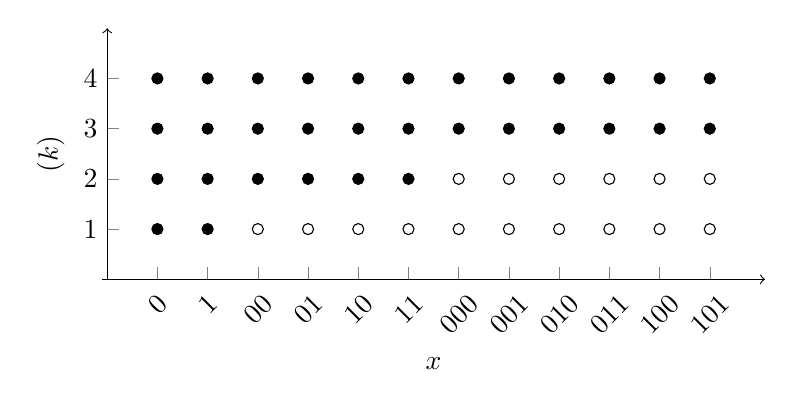
\begin{tikzpicture}
       \begin{axis}[
        width=10cm,
        axis equal image=true,
        axis lines*=middle,
        axis line style={->},
        xlabel={$x$},
        ylabel={$\asNat(k)$},
        xtick={1,2,...,12},
        xticklabels={\bits{0},\bits{1},\bits{00},\bits{01},\bits{10},\bits{11},\bits{000},\bits{001},\bits{010},\bits{011},\bits{100},\bits{101}},
        xticklabel style={rotate=45},
        ymin=0,
        ymax=5,
        ytick={1,2,...,4},
      ]
        \foreach \k in {1,2,...,4} {
          \addplot[
            only marks,
            mark=*,
            samples at={1,2,...,\k < 3 ? 2^(\k+1)-2 : 12}
          ] {\k};
          \addplot[
            only marks,
            mark=o,
            samples at={2^(\k+1)-1,2^(\k+1),...,12}
          ] {\k};
        }
      \end{axis}
    \end{tikzpicture}
    \caption{
      An initial segment of the length quasiparameterization.
      Note that the elements of the quasiparameterization, depicted as rows in the figure, are finite sets.
      Furthermore, the inclusion order on the elements of the quasiparameterization matches the natural enumeration order on the set $\binary^+$ of parameter values.
      Neither of these two properties is required to hold for an arbitrary quasiparameterization.
    }
    \label{fig:length_parameterization}
  \end{figure}
\end{example}

Quasiparameterizations are intended to also measure structures of instances other than their lengths.
Note that the length of a string is commonly associated with the symbol~$n$.
To highlight the role of quasiparameterizations as more general measures of structure, we use a similar-looking symbol for quasiparameterizations:~$\eta$.
By convention from parameterized complexity theory, we shall mostly use~$x$ for instances and~$k$ for parameter values.
The $k$th slice of a quasiparameterization~$\eta$ is denoted by~$\eta_k$.

In our framework, parameter values are mapped to sets of instances.
In this regard, our framework differs from that of~\textcite{flum2006parameterized}, where instances are mapped to parameter values.
Of course, given a quasiparameterization~$\eta$ and an instance~$x$, we can consider the set $\{k \st x \in \eta_k\}$.
These are the parameter values that the quasiparameterization~$\eta$ links to the instance~$x$.
Contrary to \citeauthor{flum2006parameterized}, we make no demands regarding the computability of such a mapping from instances to parameter values.

Recall that parameter values in the frameworks of \textcite{downey1999parameterized} and of \textcite{flum2006parameterized} are typically natural numbers.
This allows us to compare parameter values assigned to an instance by different parameterizations using the usual less-than-or-equal-to order~\parencite{komusiewicz2012new}.
In our more general framework, where instances are associated with sets of binary strings, comparing quasiparameterizations is less straightforward.
To facilitate a comparison between quasiparameterizations, we shall look at the length of the shortest parameter value for some given instance.
\begin{definition}
  Given a quasiparameterization~$\eta$, the \defkeyat{m@$\mu_\eta$}{minimization function} of~$\eta$ is defined as
  \begin{equation*}
    \mu_\eta(x) \deq \min\{\length{k} \st x \in \eta_k\}.
  \end{equation*}
\end{definition}
Note that $\mu_\eta$ minimizes with respect to the length of parameter values and not with respect to the inclusion order on the slices of the quasiparameterization.

Like in the framework of \textcite{downey1999parameterized}, in our framework an instance can be associated with multiple parameter values.
Therefore, a parameterized analysis of decision problems requires a generalization of decision procedures.
A parameterized decision procedure, or \defkeyat{parameterized procedure|(}{parameterized procedure} for short, is a special kind of procedure that takes two arguments.
In line with ordinary decision procedures, we require parameterized procedures to be total, meaning that their computation terminates on all possible inputs.
However, we do not require the output of a parameterized procedure to be either \bits{1} or~\bits{0}, representing the judgments `yes' and `no'.
Any other output a parameterized procedure produces we interpret as~\bits{?}, representing the judgment `unknown'.
In summary, a parameterized procedure is a procedure that takes two strings as input and produces an output in the set $\{\bits{1}, \bits{0}, \bits{?}\}$.\indexkey{parameterized procedure|)}

Let $\phi$ be a parameterized procedure and $\eta$ a quasiparameterization.
We say that $\phi$ \defkeyat{parameterized procedure!convergence}{converges} to a set~$A$ on~$\eta$ if, for all strings $x$ and~$k$, we have
\begin{equation*}
  x \in \eta_k \:\implies\: \phi(x, k) = A(x).
\end{equation*}
Because a quasiparameterization is consistent in the sense that it is directed, we can think of such a set~$A$ as a \emph{limit} of the parameterized procedure~$\phi$.
However, the set to which a parameterized procedure converges may depend on the quasiparameterization.
\begin{example}
\label{ex:convergence}%
  Consider the quasiparameterizations $\eta$ and~$\zeta$ given by
  \begin{equation*}
    \eta_k \deq \begin{cases}
      \binary^+	& \text{if $k = \bits{0}$}, \\
      \emptyset	& \text{otherwise},
    \end{cases}
    \qquad\text{and}\qquad
    \zeta_k \deq \begin{cases}
      \emptyset	& \text{if $k = \bits{0}$}, \\
      \binary^+	& \text{otherwise},
    \end{cases}
  \end{equation*}
  and the parameterized procedure~$\phi$ given by
  \begin{equation*}
    \phi(x, k) \deq \begin{cases}
      \bits{1}	& \text{if $k = \bits{0}$}, \\
      \bits{0}	& \text{otherwise}.
    \end{cases}
  \end{equation*}
  These definitions are so that $\phi$ converges to~$\binary^+$ on~$\eta$, but to~$\emptyset$ on~$\zeta$.
\end{example}

The above example shows that a parameterized procedure can have multiple limits.
One way to enforce the limit of a parameterized procedure to be unique is by strengthening our notion of convergence.
We do so by placing an additional requirement on quasiparameterizations.
\begin{definition}
  A \defkey{parameterization} is a point-cofinite quasiparameterization, meaning each $x \in \binary^+$ is excluded from only finitely many slices of the quasiparameterization.
\end{definition}

With parameterizations, a situation as in Example~\ref{ex:convergence} cannot occur.
A parameterized procedure~$\phi$ may converge on two different parameterizations, but the set to which $\phi$ converges will be the same either way.
In other words, as far as convergence on parameterizations is concerned, the limit of a parameterized procedure, if it exists, is unique.
Therefore, when dealing with convergence in the context of parameterizations, we need not mention a parameterization explicitly.
We may simply say that a parameterized procedure~$\phi$ converges to a set~$A$.
This then means that there exists a parameterization~$\eta$ such that $\phi$ converges to~$A$ on~$\eta$.

We remark that the length quasiparameterization of Example~\ref{ex:length_parameterization} qualifies as a parameterization.
Accordingly, we may refer to it as the \defkey{length parameterization}.
The generality of quasiparameterizations is not needed very often and for most purposes parameterizations fit the bill.
A notable exception is Section~\ref{sec:statistics}, where we shall make extensive use of quasiparameterizations in their full generality.
For computational complexity theory, parameterizations certainly suffice.
\begin{example}
  In Section~\ref{sec:parameterized_complexity_theory}, we have looked at a parameterized analysis of the \pr{Clique} problem,
  \begin{align*}
    \pr{Clique} \deq \{(G, l) \st &\text{there is a set of at least $l$ vertices of the graph $G$ in which} \\
          &\text{each pair of vertices is connected by an edge}\},
  \end{align*}
  with respect to the minimum vertex cover size.
  We found that in the framework of \citeauthor{downey1999parameterized}, such an analysis was not very natural.
  It required the construction of an intricate parameterized decision problem.

  In our framework, we can consider the unmodified \pr{Clique} problem with respect to the parameterization
  \begin{equation*}
    \eta \deq (\{(G, l) \st \text{$G$ has a vertex cover of at most $\asNat(k)$ vertices}\})_{k \in \binary^+}.
  \end{equation*}
  In the framework of \citeauthor{downey1999parameterized}, the \pr{Clique} problem parameterized by the minimum vertex cover size was found to be fixed-parameter tractable.
  For our framework, this means that there is a parameterized procedure~$\phi$ such that
  \begin{itemize}
  \item $\phi$ converges to \pr{Clique} on~$\eta$, and
  \item for some function~$f$ and constant~$c$, the running time of~$\phi$ on any instance of length~$n$ and parameter value~$k$ is at most $f(k) \cdot n^c$.
  \end{itemize}
  Thus, an analysis of fixed-parameter tractability can be performed in our framework.
  Moreover, this is possible without resorting to intricate parameterized decision problems and the parameterization can be reused for other problems.
  We remark that a more fundamental definition of fixed-parameter tractability shall be given in Section~\ref{sec:tractability:stratified}.
\end{example}

When a parameterized procedure~$\phi$ converges to some set on a parameterization~$\eta$, the set to which $\phi$ converges does not depend on the specifics of~$\eta$.
Suppose that $\phi$ converges to a set~$A$.
This does not mean that whenever for some instance~$x$ and parameter value~$k$ we have $\phi(x, k) = \bits{1}$, we can conclude that $x$ is a member of~$A$.
Likewise, whenever we have $\phi(x, k) = \bits{0}$, we cannot conclude that $x$ is not a member of~$A$.
All we know is that for each instance~$x$ there are only finitely many parameter values~$k$ such that $\phi(x, k)$ is not in agreement with membership of~$x$ in~$A$.
In other words, we do not \emph{know} when the output of~$\phi$ is correct, only that it will eventually be correct.
Of particular importance are the parameterized procedures of which we do know when they are correct.
These are the parameterized procedures~$\phi$ for which
\begin{equation*}
  (\{x \st \phi(x, k) \neq \bits{?}\})_{k \in \binary^+}
\end{equation*}
is a parameterization on which $\phi$ converges to some set~$A$.
In particular, for all instances~$x$ and parameter values~$k$, we have that $\phi(x, k)$ is either \bits{?} or $A(x)$.
We call such parameterized procedures \defkeyat{parameterized procedure!direct}{direct}.

When the parameter value is held fixed, the behavior of a direct parameterized procedure can be thought of as an approximation of a decision procedure.
Indeed, such procedures are of interest also without any parameter values playing a part.
\begin{definition}
\label{def:approximation}%
  Given a function $t$, a procedure~$\phi$ is a \defkeyat{approximation@$t$-approximation}{$t$"~approximation} for a set~$A$ if it satisfies, for every string~$x$,
  \begin{itemize}
  \item $\phi(x)$ outputs either \bits{?} or $A(x)$, and
  \item $\phi$ terminates on input $x$ within $t(\length{x})$ steps.
  \end{itemize}
  A $t$"~approximation~$\phi$ is said to \emph{decide} the elements of its \defkeyat{approximation@$t$-approximation!domain}{domain}
  \begin{equation*}
    \dom(\phi) \deq \{x \st \phi(x) \neq \bits{?}\}.
  \end{equation*}
\end{definition}

The \defkeyat{approximation@$t$-approximation!polytime}{polytime-approximations} \parencite{ko1981completeness,balcazar1985bi-immune} are $t$"~approximations where $t$ is a polynomial.
Likewise, a procedure is an \defkeyat{approximation@$t$-approximation!O(f)@$\bigO(f)$}{$\bigO(f)$"~approximation} if it is a $t$"~approximation for some $t \in \bigO(f)$.
The fact that the bound is a bound on the running time is left implicit.
For time-constructible functions~$t$, the domain of a $t$"~approximation is decidable in time~$t$.
In particular, the domain of a polytime-approximation is in \cl{P}, without an increase in the degree of the polynomial.
The domain of a polytime-approximation is also known as the \emph{definite part} of the approximation~\parencite{ko1981completeness}.

